\chapter{Checklist Management}

\section{Overview}

The Checklist Management system in KanardiaCloud allows pilots and aviation professionals to create, organize, and print professional digital checklists. These checklists can be synchronized with Kanardia devices and printed in various formats for cockpit use.

\begin{figure}[H]
\centering
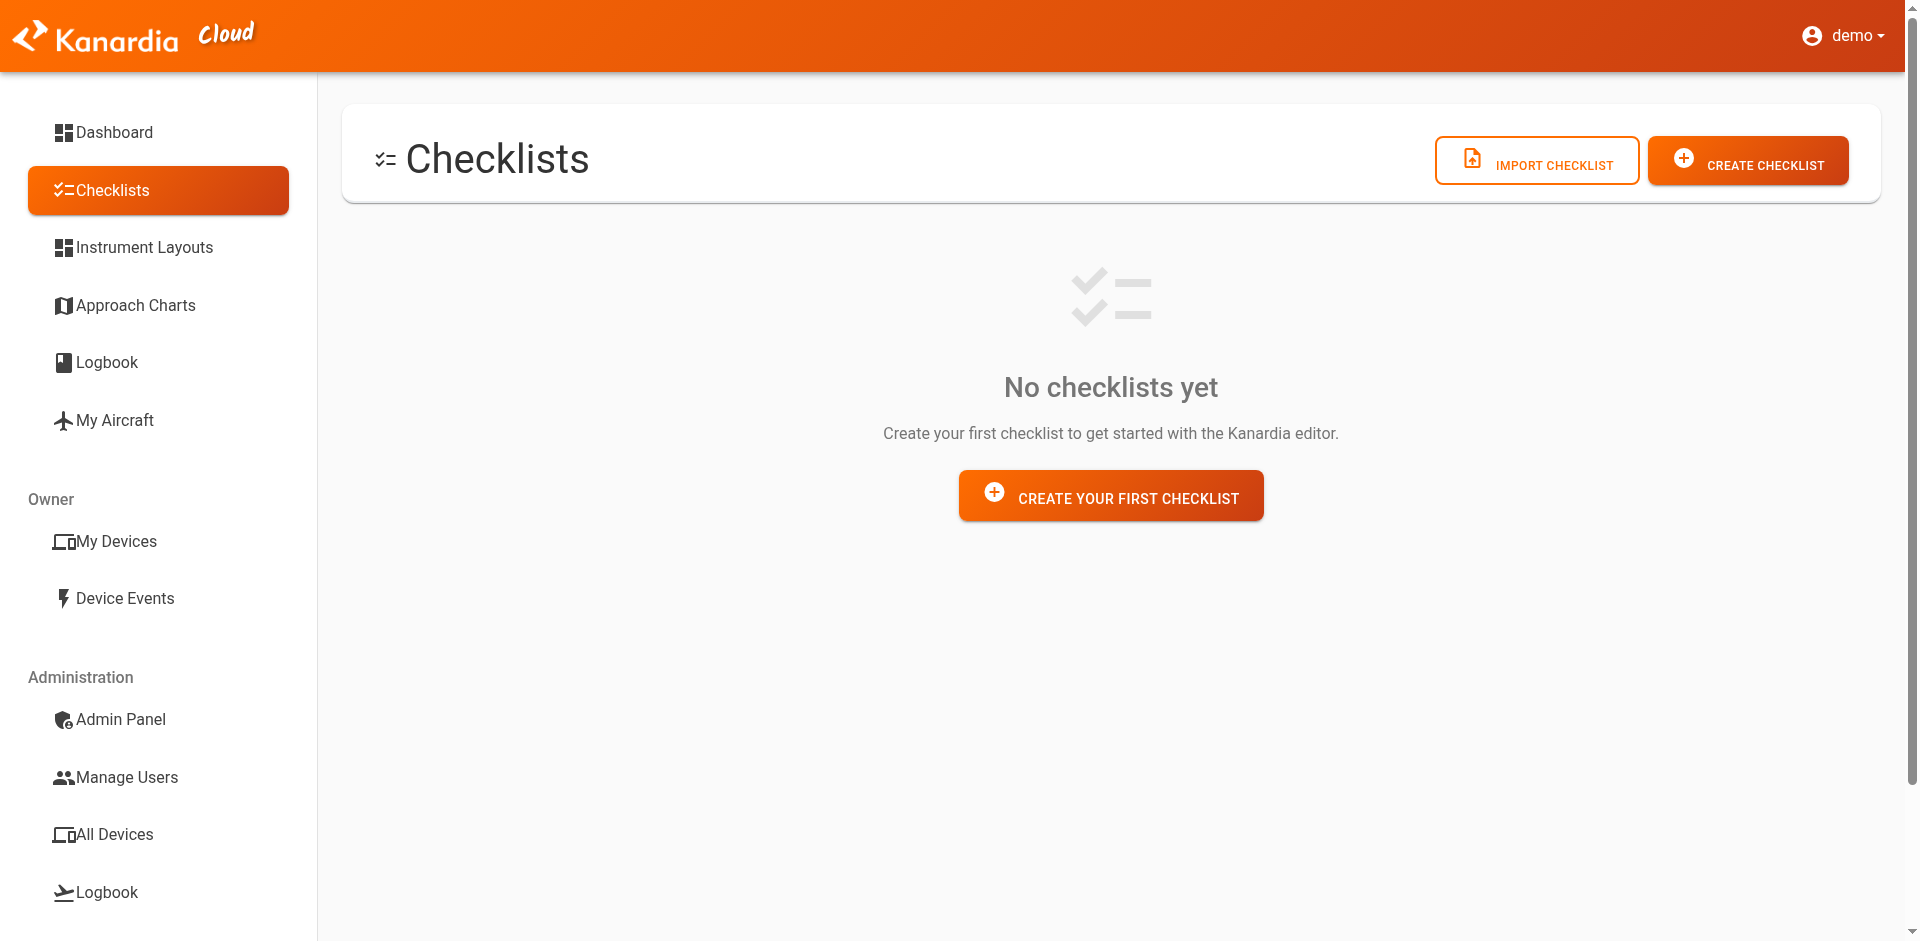
\includegraphics[width=\textwidth]{images/checklist_dashboard.png}
\caption{Checklist Management Dashboard}
\label{fig:checklist_dashboard}
\end{figure}

\section{Creating Checklists}

\subsection{New Checklist Creation}

To create a new checklist:

\begin{enumerate}
    \item Navigate to \textbf{Checklists} in the main menu
    \item Click the \textbf{"Create New Checklist"} button
    \item Fill in the basic information:
    \begin{itemize}
        \item \textbf{Title}: Descriptive name for the checklist
        \item \textbf{Description}: Optional detailed description
        \item \textbf{Aircraft Type}: Associated aircraft model (if applicable)
    \end{itemize}
    \item Click \textbf{"Create Checklist"} to proceed to the editor
\end{enumerate}

\begin{figure}[H]
\centering
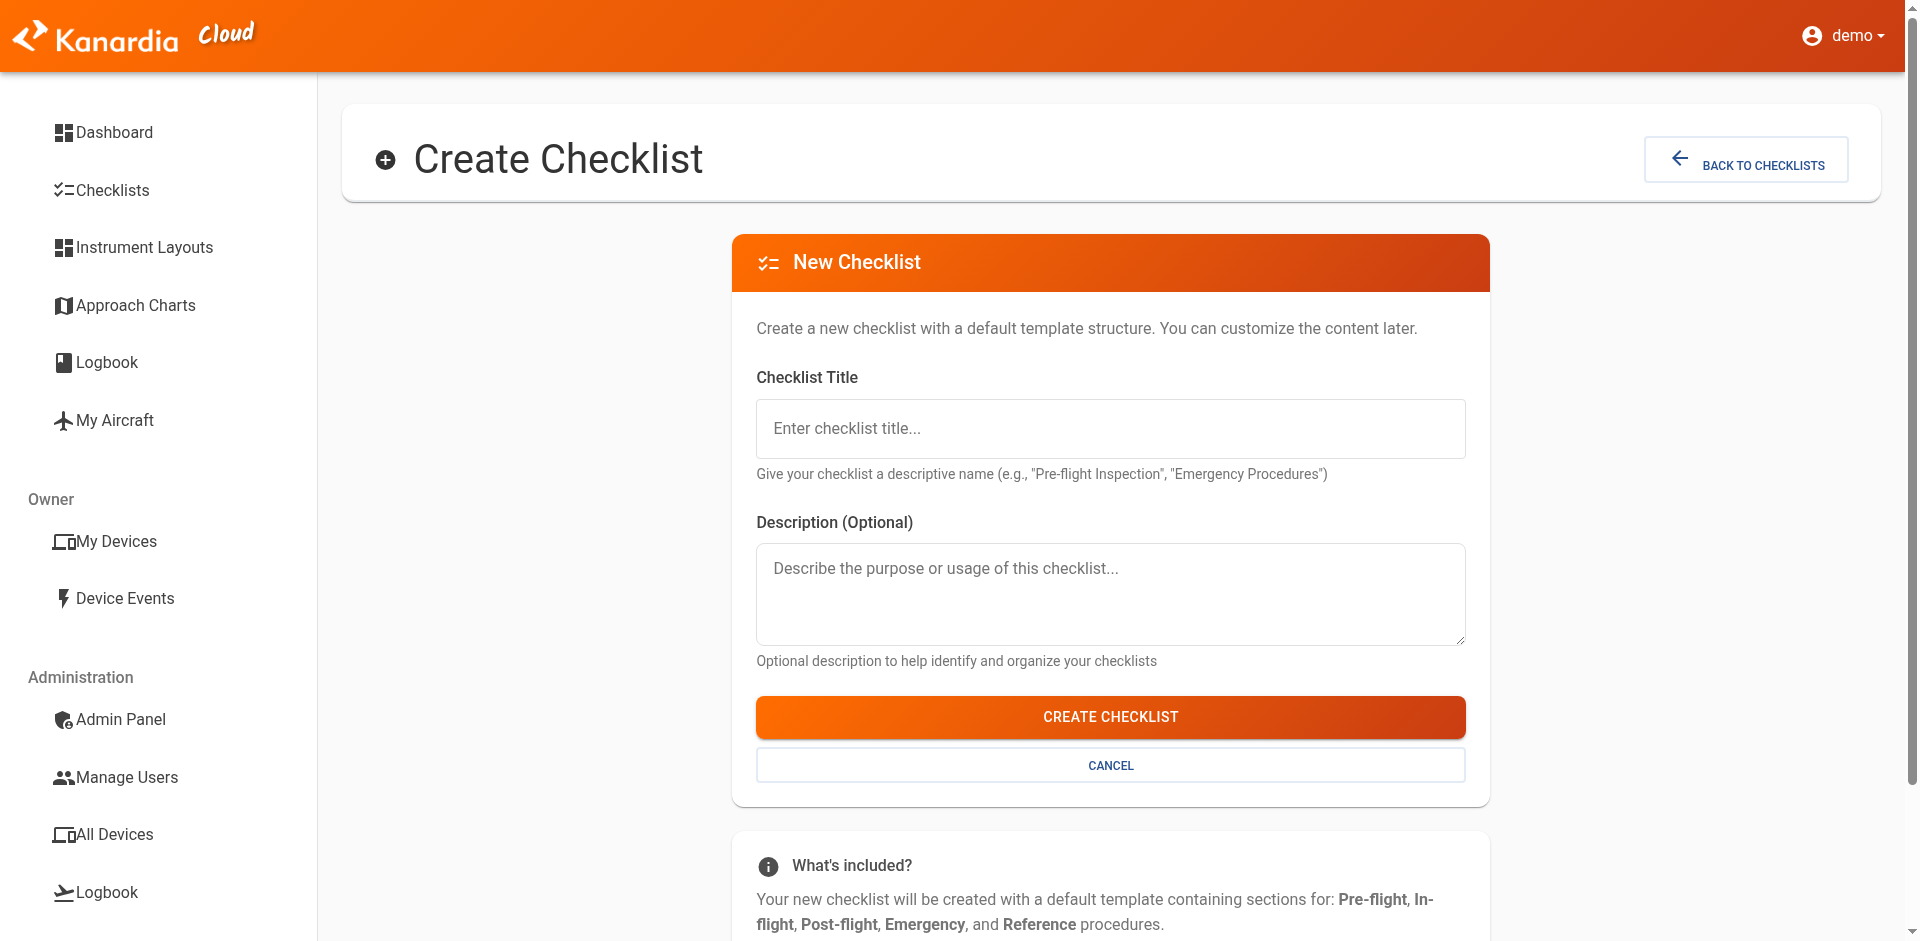
\includegraphics[width=0.8\textwidth]{images/create_checklist_form.png}
\caption{New Checklist Creation Form}
\label{fig:create_checklist_form}
\end{figure}

\subsection{Checklist Structure}

KanardiaCloud checklists are organized hierarchically:

\begin{description}
    \item[Root] Top-level container for the entire checklist
    \item[Sections] Major groupings (e.g., "Pre-flight", "Engine Start", "Landing")
    \item[Checklists] Individual procedures within sections
    \item[Items] Specific actions or checks within each checklist
\end{description}

\section{Checklist Editor}

\subsection{Editor Interface}

The checklist editor provides a comprehensive interface for building detailed checklists:

\begin{itemize}
    \item \textbf{Tree View}: Hierarchical structure on the left
    \item \textbf{Properties Panel}: Item details on the right
    \item \textbf{Toolbar}: Quick actions and tools
    \item \textbf{Preview}: Real-time preview of changes
\end{itemize}

\begin{figure}[H]
\centering

\includegraphics[width=\textwidth]{images/checklist_editor.png}
\caption{Checklist Editor Interface}
\label{fig:checklist_editor}
\end{figure}

\subsection{Adding Sections and Items}

To add new elements to your checklist:

\begin{enumerate}
    \item \textbf{Adding a Section}:
    \begin{itemize}
        \item Right-click on the root node or use the "Add Section" button
        \item Enter the section name (e.g., "Pre-flight Inspection")
        \item Set section properties if needed
    \end{itemize}
    
    \item \textbf{Adding a Checklist}:
    \begin{itemize}
        \item Right-click on a section or use "Add Checklist"
        \item Name the checklist (e.g., "External Inspection")
        \item Configure checklist properties
    \end{itemize}
    
    \item \textbf{Adding Items}:
    \begin{itemize}
        \item Right-click on a checklist or use "Add Item"
        \item Enter the item title and action
        \item Set item properties and responses
    \end{itemize}
\end{enumerate}

\subsection{Item Properties}

Each checklist item can be configured with:

\begin{table}[H]
\centering
\begin{tabular}{@{}lp{8cm}@{}}
\toprule
\textbf{Property} & \textbf{Description} \\
\midrule
Title & The main text of the checklist item \\
Action & Expected response or action to take \\
Type & Item type (check, action, warning, etc.) \\
Priority & Item importance level \\
Notes & Additional information or remarks \\
Voice & Text-to-speech pronunciation guide \\
\bottomrule
\end{tabular}
\caption{Checklist Item Properties}
\label{tab:item_properties}
\end{table}

\section{Checklist Import and Export}

\subsection{Supported Formats}

KanardiaCloud supports various checklist formats:

\begin{itemize}
    \item \textbf{Kanardia CKL}: Native Kanardia checklist format
    \item \textbf{JSON}: Standard JSON format for data exchange
    \item \textbf{XML}: Structured XML format
    \item \textbf{CSV}: Simple comma-separated values (basic import only)
\end{itemize}

\subsection{Importing Checklists}

To import an existing checklist:

\begin{enumerate}
    \item Go to \textbf{Checklists} $\rightarrow$ \textbf{Import}
    \item Select the file format
    \item Choose the checklist file
    \item Review the import preview
    \item Confirm the import
    \item Edit as needed using the checklist editor
\end{enumerate}

\begin{figure}[H]
\centering
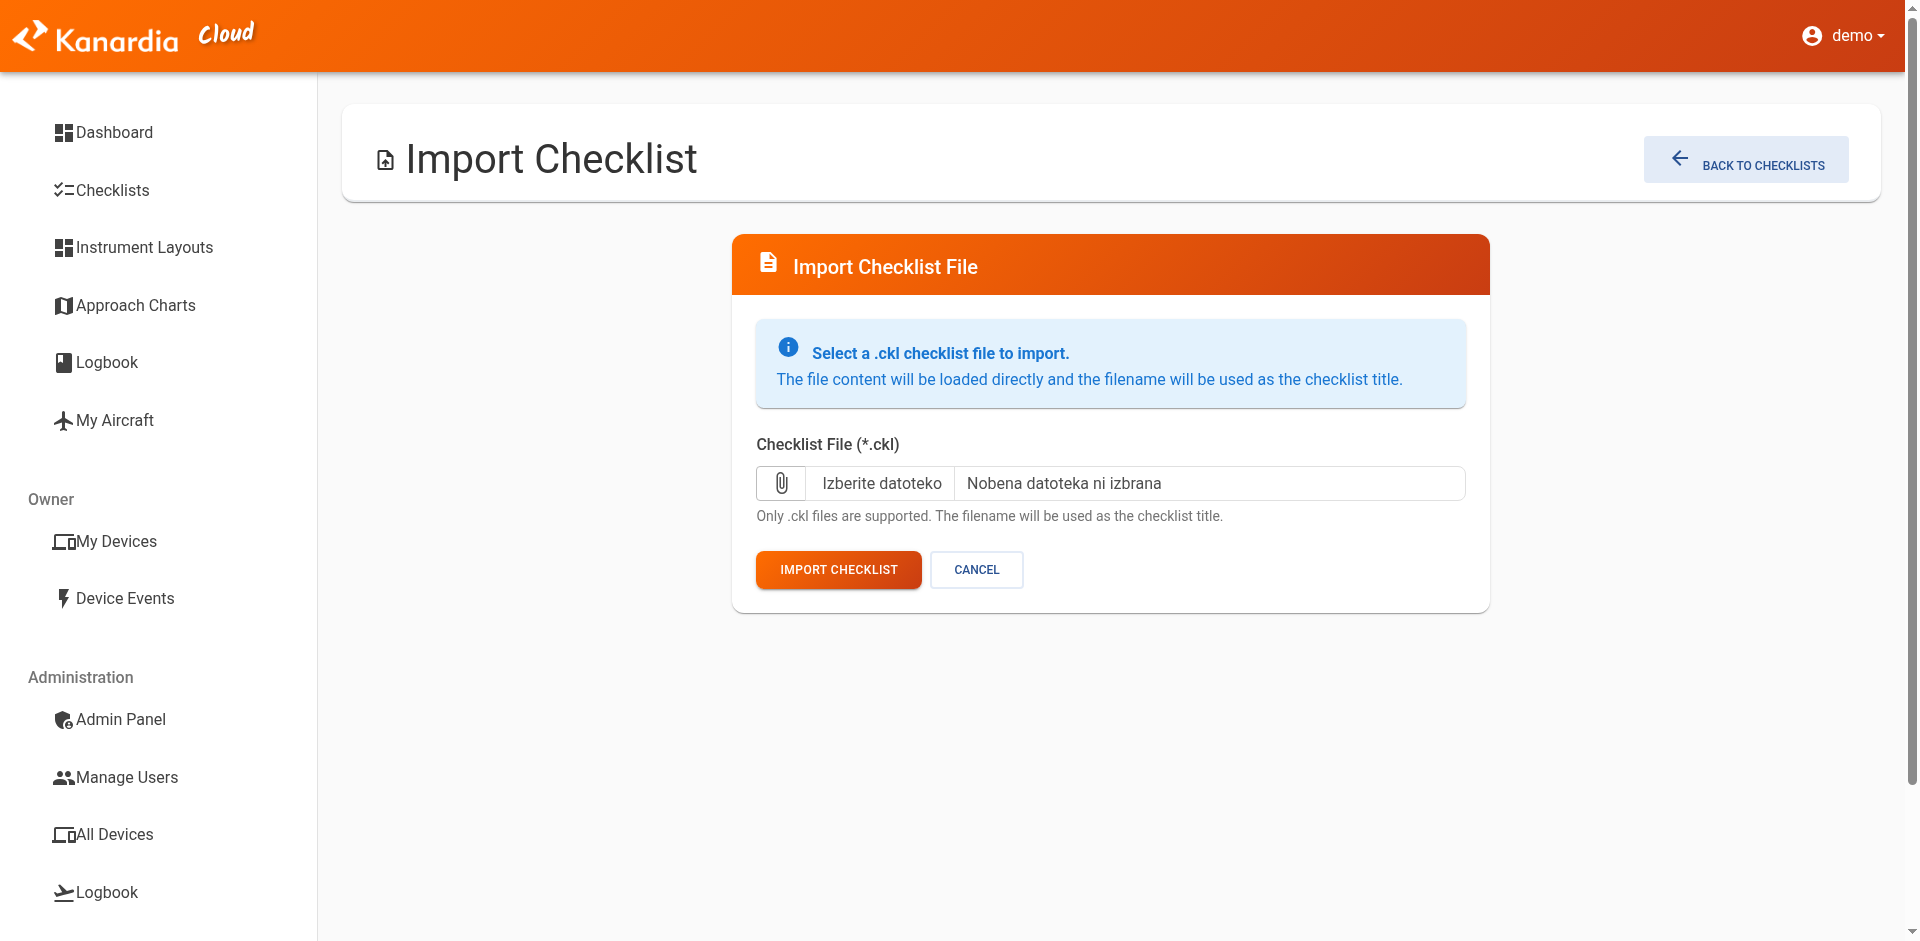
\includegraphics[width=0.8\textwidth]{images/checklist_import.png}
\caption{Checklist Import Interface}
\label{fig:checklist_import}
\end{figure}

\subsection{Exporting Checklists}

To export a checklist:

\begin{enumerate}
    \item Open the checklist you want to export
    \item Click the \textbf{"Export"} button in the toolbar
    \item Select the desired format
    \item Choose export options
    \item Download the exported file
\end{enumerate}

\section{Printable Checklists}

\subsection{Print Formats}

KanardiaCloud offers two optimized print formats:

\subsubsection{Standard Format}
\begin{itemize}
    \item Full page layout with headers and metadata
    \item Section titles prominently displayed
    \item Two-column layout for efficient paper use
    \item Complete checklist information included
\end{itemize}

\subsubsection{Minimal Format}
\begin{itemize}
    \item Compact layout without headers
    \item All checklists on one page
    \item Section names shown on each card
    \item Optimized for cockpit reference
\end{itemize}

\begin{figure}[H]
\centering
\begin{subfigure}[b]{0.48\textwidth}

\includegraphics[width=\textwidth]{images/checklist_print_standard.png}
\caption{Standard Print Format}
\label{fig:print_standard}
\end{subfigure}
\hfill
\begin{subfigure}[b]{0.48\textwidth}

\includegraphics[width=\textwidth]{images/checklist_print_minimal.png}
\caption{Minimal Print Format}
\label{fig:print_minimal}
\end{subfigure}
\caption{Checklist Print Formats}
\label{fig:print_formats}
\end{figure}

\subsection{Accessing Print Versions}

To generate printable checklists:

\begin{enumerate}
    \item Navigate to your checklist
    \item Click the options menu (three dots)
    \item Select \textbf{"Printable Version"}
    \item Choose between Standard or Minimal format
    \item Use browser print function or click \textbf{"Print Checklist"}
\end{enumerate}

\subsection{Print Optimization}

Both print formats are optimized for:
\begin{itemize}
    \item Standard A4 and Letter paper sizes
    \item Two-column layout for space efficiency
    \item Clear, readable fonts suitable for cockpit lighting
    \item Professional appearance with Kanardia branding
    \item Page breaks that avoid splitting checklists
\end{itemize}

\section{Checklist Organization}

\subsection{Categories and Tagging}

Organize your checklists using:

\begin{itemize}
    \item \textbf{Categories}: Group by aircraft type, operation type, etc.
    \item \textbf{Tags}: Custom labels for flexible organization
    \item \textbf{Favorites}: Mark frequently used checklists
    \item \textbf{Recent}: Quick access to recently modified items
\end{itemize}

\subsection{Search and Filtering}

Find checklists quickly using:

\begin{itemize}
    \item \textbf{Text Search}: Search titles and content
    \item \textbf{Category Filters}: Filter by assigned categories
    \item \textbf{Date Filters}: Show recently created or modified
    \item \textbf{Status Filters}: Filter by completion or approval status
\end{itemize}

\section{Collaboration and Sharing}

\subsection{Sharing Checklists}

Share checklists with team members:

\begin{enumerate}
    \item Open the checklist to share
    \item Click \textbf{"Share"} in the toolbar
    \item Enter recipient email addresses
    \item Set permission levels (view, edit, admin)
    \item Add an optional message
    \item Click \textbf{"Send Invitation"}
\end{enumerate}

\subsection{Version Control}

KanardiaCloud maintains checklist versions:

\begin{itemize}
    \item Automatic version history
    \item Compare different versions
    \item Restore previous versions
    \item Track changes and modifications
    \item Comment on changes
\end{itemize}

\section{Best Practices}

\subsection{Checklist Design}

Follow these guidelines for effective checklists:

\begin{itemize}
    \item \textbf{Clear Language}: Use precise, unambiguous terms
    \item \textbf{Logical Flow}: Arrange items in operational sequence
    \item \textbf{Consistent Format}: Maintain uniform structure
    \item \textbf{Appropriate Length}: Keep individual checklists manageable
    \item \textbf{Regular Updates}: Review and update periodically
\end{itemize}

\subsection{Naming Conventions}

Use consistent naming for easy identification:

\begin{itemize}
    \item Include aircraft type in title
    \item Use standard aviation terminology
    \item Follow company or organizational standards
    \item Include version numbers or dates
\end{itemize}

\subsection{Testing and Validation}

Before using checklists operationally:

\begin{itemize}
    \item Review with experienced pilots
    \item Test in simulator environments
    \item Validate against official procedures
    \item Check for completeness and accuracy
    \item Obtain necessary approvals
\end{itemize}

\section{Troubleshooting}

\subsection{Common Issues}

\begin{description}
    \item[Import Failures] Check file format and encoding, ensure file is not corrupted
    \item[Print Layout Issues] Verify browser print settings, try different browsers
    \item[Sync Problems] Check device connection, verify account permissions
    \item[Missing Items] Refresh page, check filter settings, verify data integrity
\end{description}

\subsection{Getting Help}

If you encounter issues with checklist management:

\begin{itemize}
    \item Check the built-in help tooltips
    \item Review this user manual
    \item Contact support with specific error messages
    \item Provide checklist files for technical analysis
\end{itemize}
